\section{Introduction}

%% 
%% Leave first page empty
\thispagestyle{empty}

The need of a new way to communicate between two points of the planet is a problem that many different technologies have tried to approach. Systems such Skype or VoIP are not able to cope the needs of the new generations of developers and users that everyday require a more integrated way of communication with the World Wide Web (WWW). 

Besides this, the amount of data transferred during the last years and the prevision for the future allocates a new scenario where non-centralized systems such as P2P are required as data bandwidth grows and systems need to become more scalable. Nowadays, networks are still manly content-centric, meaning that data is provided from a source to a client in a triangle scheme, clients upload data to central servers and this data is transferred to the endpoint. This architecture has been provided since long time as reliable and scalable, but with the appearance of powerful applications and Video On Demand (VOD) scalability is becoming an issue.

Those circumstances lead to a whole new world of real-time browser based applications which require also a new framework to work with. Ranging from online videoconferencing to real-time data applications, for this purpose few attempts were made in the past being highly reliable on specific hardware and custom-built no-compatible systems. Those proposals were not accessible to normal users that could not afford to adapt the requirements. 

All previous concepts are now possible thanks to the increase of the average performance in every computer nowadays, this situation is helping to build more complex browsers that are able to perform many different tasks that enhance web browsing to a different level. Having a browser to handle OpenGL style of applications is now possible thank to the new  HyperText Markup Language version 5 (HTML5) standard. Multimedia abilities are also able to be reproduced on those browsers and webcam media shown as HTML is now a reality. Even dough, there is still an important issue that must be addressed: there is no common standardized protocol that allows developers to do this. Web Real-Time Communication (WebRTC) effort to approach this problem is to build a simple and standard solution for peer-to-peer browser communication in the HTML5 environment~\cite{alvestrandOverview2012} .

Internet bandwidth capabilities helped to take the decision to start integrating peer-to-peer solutions in browsed based applications, this is due the year-by-year increase of user bandwidth connectivity during the last 10 years. Actual latency in the network is low enough to allow real-time applications to work resiliently in the browser. The amount of users being able to transfer at high speed has increased during last years (Figure~\ref{fig:bwWorldAvg}), about 39\% of users are able to download at speeds greater than 4Mbps being this a very good average speed for multimedia content~\cite{akamaiq2}.

\begin{figure}[h]
  \centering
    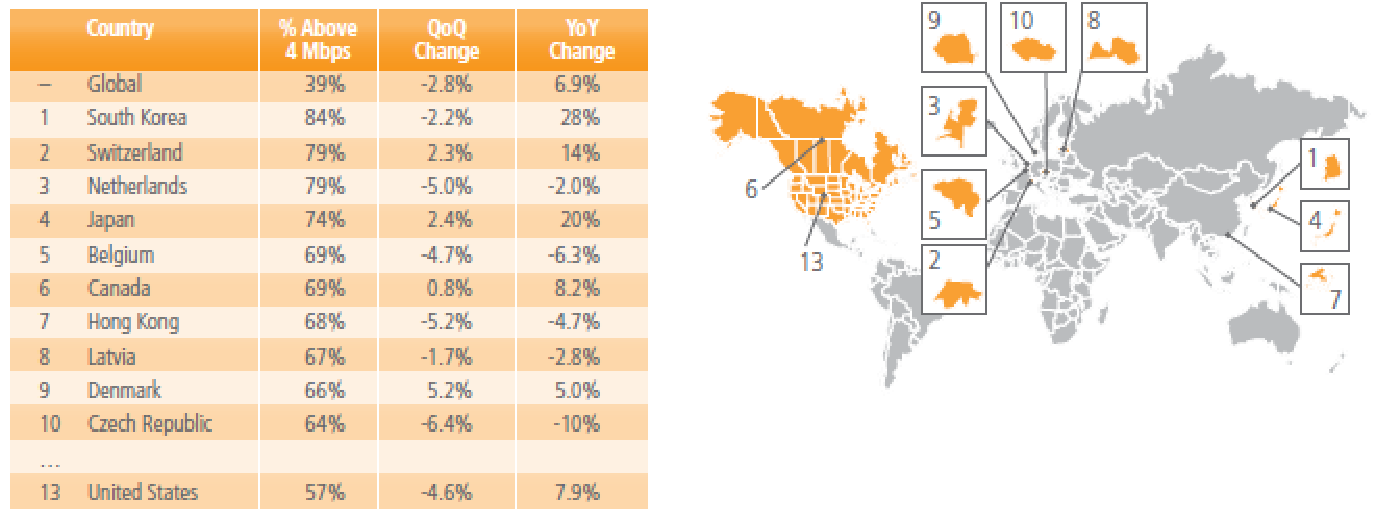
\includegraphics[width=1\textwidth]{./figures/internetstats.pdf}
      \caption[Broadband over 4Mbps connectivity statistics]{Broadband connectivity statistics about the speeds over 4Mbps around the globe.}
	\label{fig:bwWorldAvg}
\end{figure}

Regarding the specs on the client side, recent surveys and statistics taken by the game manufacturer Steam prove that more than  61\% of machines are carrying 1 to 4 gigabytes of RAM and nearly 90\% of computers handle 2 to 4 core CPU with a 64 bit OS~\cite{steamStats}, this environment can easily handle media enhanced applications that require high performance for media encoding. WebRTC concept rests over multiple layers having the browser as an underlying application, a traditional browser allocates a lot of resources for running being the performance of the machine a bottleneck in some cases.

Traditionally, WebRTC concept approaches rely on the usage of plug-ins or other separate software components that make the system run smoother by avoiding one layer of processing (browser) but being non-standard and not cross-compatible, one of the most import ant concepts when designing applications nowadays. This approach has a new alternative with the arrival of the new HTML5 where WebRTC is integrated as one of the new Application Programming Interfaces (APIs) available alongside other many different interesting capabilities.

\subsection{Background}

WebRTC API is included into the HTML5, this is the fifth version of the WWW language. This version includes different API's and JavaScript codes that help the developer to easily introduce new features into their already existing WWW applications. The initial HTML version (2.0) was published in November 1995 with the only goal of delivering static content from the server to client browser~\cite{html2IETF}. HTML became de de facto format for serving web information. 

HTML is written in tag formatting to identify different elements. Those tags are then interpreted by the browser to show the different data content served by the server. During the evolution of the WWW different new features have been added to the HTML standard and new versions where published, things like JavaScript and Style Sheets increase the flexibility and features of the WWW content enhancing the final user experience.

Due to the need to extend the features of the already existing HTML4 standard, a new version was proposed in 2004 by the Mozilla Foundation and Opera Software~\cite{initialHTML5proposition}. This new proposition focused in new developing technologies that could be backwards compatible with the already existing browsers, the idea didn't make a success and was tier apart until January 2008 when the first Public Working Draft was published by the Web HyperText Application Technology Working Group (WHATWG) in the W3C~\cite{firstHTML5draft}.

This proposal had a greater reliance in modularity in order to move forward faster, this meant that some specs that were included in the initial draft moved to different working groups in the W3C. Those technologies defined in HTML5 are now in separate specifications, one of them being WebRTC. WebRTC works as an integrated API within the browser that is accessible using JavaScript and is used in conjunction with the Document Object Model (DOM) interfaces. Some of the APIs that have been developed are not part of the HTML5 W3C specification but are included into the WHATWG HTML specification.

\subsection{Contribution}

Investigate how WebRTC performs in a real environment trying to evaluate the best way to set multiple peer connections able to transfer media and data in different network topologies. Measure the performance of WebRTC in a real environment identifying bottlenecks related to encoding/decoding, media establishment or connection maintenance. All this should be performed in real-time over a browser by using the already existing WebRTC API.

Using metrics related to RTT, latency, packet loss and bandwidth usage we expect to understand the way WebRTC performs when handling multiple connections.

\subsection{Goals}

WebRTC uses and adapts some existing technologies for real-time communication. This thesis will focus in studying how:

\begin{itemize}
	\item WebRTC performs considering different topologies using video/audio acquired form the Webcam using the API and encoded using different codec types provided by the standard.

	\item Usage of WebRTC to build a real application that can be used by final users proving that the API is ready to be deployed and is a good approach for the developer needs when building real-time applications over the web. This will be done in conjunction with other new APIs and technologies introduced with HTML5.
\end{itemize}

The final conclusion will cover an overall opinion and usage experience of WebRTC, providing some valuable feedback for the needs and requirements for further modifications on the API.

\subsection{Structure}

Not sure about here